\documentclass[document.tex]{subfiles}
\begin{document}

\chapter {Prototypes}
\label {ch:prototypes}

In order to select a workflow framework for use in the project, a simple prototype application was constructed in both Ruote and Stonepath. The prototype application is designed around features that seemed like a good fit for the capabilities of workflow frameworks, rather than any real-world use case.


\sectionnote {BM}
\section {Overview of the Prototype Application}
\label {sec:overview-of-the-prototype-application}

\todo {Drop the reference, and specify what criteria we were evaluating in-line}

The prototype application was designed to encompass as many of the criteria in section \ref{sec:evaluation-questions} as possible in a small demonstration application. A somewhat contrived issue tracking system was designed to match these criteria.

The issue tracking system has three classes of users: reporters, developers, and project managers. Reporters are users who are responsible for reporting bugs, and providing information more information on request. Developers claim bugs from the pool of open issues, implement a fix, and then sign off on the issue. Project managers consult with developers and reporters, and assign a deployment date for the fix. All classes of users can view and comment on bugs, though they are restricted to perform only the following actions:
\begin{itemize}
\item reporters may only create issues;
\item developers may only claim issues that have not yet been claimed, and can only sign off on issues that they have claimed; and
\item project managers may only set the deployment date on issues.
\end{itemize}

Once a developer has signed off on an issue, and a project manager has set a deployment date, the issue is closed. Developers and project managers may sign off and set deployment dates in any order - though this is a somewhat unrealistic requirement, it is a good example of a pair of parallel activities. Finally, if a developer holds an issue for a week with, then the issue reverts to an unclaimed state.


\sectionnote {BM}
\section {Stonepath Prototyping Results}
\label {sec:stonepath-prototyping-results}

The requirements for the issue tracking system were translated into the state machine in Figure \ref{fig:stonepath-prototype-state-machine}. The state machine corresponds to the state of an issue - each action taken by a developer or product manager on an issue has an equivalent event. A developer claiming an issue generates a \verb!claim! event, while a developer signing off on an issue or a project manager setting the deployment date generates a \verb!close! event. As both a sign off and a deployment date are necessary for an issue to be closed, the closed state is guarded by the \verb!completed?! method.

\begin{figure}[!ht]
\centering \includegraphics[height=5in]{./img/prototypes/stonepath-state-machine}
\caption{State chart for issues in the prototype issue tracking system described in section \ref{sec:overview-of-the-prototype-application}}
\label{fig:stonepath-prototype-state-machine}
\end{figure}

The state machine model also includes a \verb!timeout! event which is triggered seven days after the in progress state is entered. The timeout was omitted from the prototype to save time, as it was not considered a risk -- several libraries already exist for Rails that provide delayed execution of method calls, as is discussed further in section \ref{sec:4ys-handling-deadlines}.

Additionally, the model also includes actions to create and destroy tasks when appropriate. Though this appeared to the be correct way to model participation in a workflow when the state machine was designed, it was discarded in the implementation, as described below.

The state machine was translated to a Ruby on Rails application, which is available at \url{https://github.com/WorkflowsOnRails/stonepath-timeboxed-example}. The application was implemented from the bottom up. First a workitem was implemented for issues, as demonstrated in the code snippet in Figure \ref{fig:stonepath-prototype-workitem}. Next, workbenches were created to for roles and users. Finally, a generic task type was defined to associate workitems and workbenches. After the model was completed, Devise was integrated to handle authentication, and the model was wrapped with appropriate views and controllers to drive the application.

\todo {Mention Devise and Cancan only in passing, making forward references to the case study for more information.}

\begin{figure}[!ht]
  \begin{lstlisting}
class Issue < ActiveRecord::Base
  include StonePath::WorkItem
  owned_by :user  # owned by the initial reporter
  tasked_through :task
  state_machine do
    state :pending, initial: true,
      after_enter: [:create_claim_task, :create_deploy_task],
      after_exit: :destroy_claim_task
    state :in_progress, after_enter: :create_develop_task,
      after_exit: :destroy_develop_task
    state :closed, after_enter: :destroy_deploy_task

    event :claim do
      transitions from: :pending, to: :in_progress
    end

    event :timeout do
      transitions from: :in_progress, to: :pending
    end

    event :close do
      transitions from: :in_progress, to: :closed, guard: :completed?
    end
  end

  def completed?
    signed_off and deployment_date.present?
  end

  # ... other scopes, associations, validations and methods ...
end
  \end{lstlisting}
  \caption{Implementation of the state machine from Figure \ref{fig:stonepath-prototype-state-machine} as a Stonepath work item}
  \label{fig:stonepath-prototype-workitem}
\end{figure}

The prototype identified several possible areas of improvement for both Rails and Stonepath projects, such as:

\paragraph{Pre-populated roles:} each role in the application was modelled with an instance of the \verb!Role! model. This allowed work items to be assigned to logical groups of users, but required extra work to put roles into the database. A seed migration had to be run whenever a production or test database was set up to create the roles, or else the application could not work. If the case studies use this approach to model roles, we will need a reusable way to specify the roles in the model and have them automatically populated in the database.

\paragraph{Authorization:} though Stonewall is advertised as a flexible authorization layer that integrates well with Stonepath, its permissions are much too finely grained to be useful. Stonewall sets permissions at the method level, while access controls are usually described in terms of actions that users can perform, instead of individual attributes they can access and set. In the end, a custom solution was created, which evolved to check users against an approved list of roles in each controller action in Rails. This technique matched almost one-to-one to the actions described in the requirements. Fortunately, Cancan already implements a similar action-based approach, and is also able to centralize access controls to a single source file instead of hard-coding them in each action.

\paragraph{Task modelling:} though the task model in Figure 1 was straightforward to design, it was unwieldy in practice. Stonepath represents each task as a Rails model with a polymorphic association to a workbench and a workitem. Unfortunately, polymorphic associations are implemented in Rails, and not at the database level, so it is difficult to request the developer assigned to an issue by querying the tasks. On the other hand, a developer column on an issue is easy to understand and query. Additionally, tasks are heavyweight - each task includes its own state machine, which went totally unused in the prototype application. Tasks seem to be best used to model sub-activities of an activity, while associations that need to be queried should be added to the work item itself.


\FloatBarrier

\sectionnote {AC}
\section {Ruote Prototyping Results}
\label {sec:ruote-prototyping-results}

The BPMN model shown in Figure \ref{fig:ruote-bpmn-diagram} describes how the issue tracking system works using process based methodologies. The workflow of a report begins when it is created and joins the unclaimed report pool. Developers are then able to claim the report and Managers are able to set the deployment date. Once both actions have been accomplished the developer is able to sign off the report which will then close. If the report has not been signed off after 7 days the report returns to the unclaimed report pool.

Reporters are only able to create new reports. Developers are only able to claim unclaimed reports and sign off on the reports that they have claimed. Managers are only able to assign deployment dates to each report.

\begin{figure}[!ht]
\centering 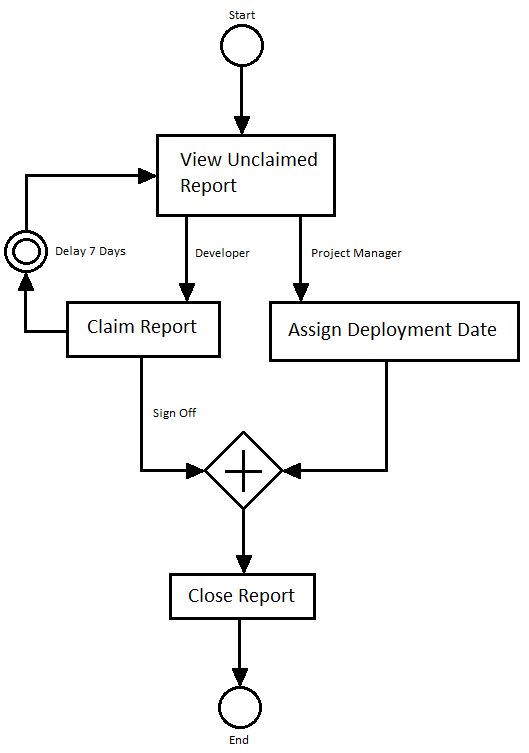
\includegraphics[height=5in]{./img/prototypes/ruote-bpmn-diagram}
\caption{BPMN for the Ruote prototype issue tracking system.}
\label{fig:ruote-bpmn-diagram}
\end{figure}

\paragraph{Ruote-Kit:} provides an easy way of accessing the Ruote dashboard and handles all of the Ruote rails routes. The dashboard is the core of Ruote providing access to the many processes, participants, and workers. A process can be considered the entire workflow, and the participants can be considered the events within the workflow. Ruote-Kit automatically creates a default dashboard object and populates it with a default worker. Workers in Ruote are threads which are used by the participants to do operations on the workitem. The workitem is passed between participants and in the case of this application is the report.

\paragraph{Participants:} Participants contain the logic that is executed whenever a process definition reaches it. Each participant is created using its own class located in app\slash participants. When a participant is called by a process definition it executes its \verb!on_workitem! method. The participant must call 'reply' to notify the process that it has finished working on an item. The basic outline of a participant is shown in Figure \ref{fig:ruote-prototype-participant-code}.

\begin{figure}[!ht]
  \begin{lstlisting}
class UnclaimedPoolParticipant
  include Ruote::LocalParticipant

  def on_workitem
    # the report_id is passed between participants and stored
    # in the workitem
    report = Report.find(workitem.lookup(id))
    --- do work on the report here ---
    reply #call to the process to notify work has finished
  end

  def on_cancel
    #called when workitem is canceled
  end

  def on_error
    #called when an error occurs
  end
end
  \end{lstlisting}
  \caption{The framework of a participant class and its methods.}
  \label{fig:ruote-prototype-participant-code}
\end{figure}

In order to use a participant in a process definition Ruote must be able to find your participant class. This is done in an initializer file so that the participants are registered and ready for use when the server is started. The method of registering participants with Ruote is shown below in Figure \ref{fig:ruote-prototype-participant-register}.

\begin{figure}[!ht]
  \begin{lstlisting}
#Register each participant for use in a process definition
RuoteKit.engine.register do
  participant 'unclaimed_pool', UnclaimedPoolParticipant
  participant 'claim_issue', ClaimIssueParticipant
  participant 'sign_issue', SignIssueParticipant
  participant 'close_issue', CloseIssueParticipant
end
  \end{lstlisting}
  \caption{Registering the participants with the Dashboard.}
  \label{fig:ruote-prototype-participant-register}
\end{figure}

\paragraph{Process:} A process is created along side every new Report and the work item is set to the newly created report. Figure \ref{fig:ruote-prototype-process-definition} displays the process definition and the participants used to model the BPMN diagram in Figure \ref{fig:ruote-bpmn-diagram}.

\begin{figure}[!ht]
  \begin{lstlisting}

-- REPORT_OBJECT is created up here and the model is saved

pdef = Ruote.process_definition do
  unclaimed_pool
  concurrent do
    claim_issue
    sign_issue
  end
  close_issue
end

RuoteKit.engine.launch(pdef, REPORT_OBJECT) #launches the process

  \end{lstlisting}
  \caption{Process Definition of the Ruote prototype bug tracker.}
  \label{fig:ruote-prototype-process-definition}
\end{figure}

This process definition first calls the \verb!on_workitem! method in the \verb!unclaimed_pool! participant and waits for a reply call to notify that the \verb!on_workitem! method has finished executing. Once it has finished execution \verb!claim_issue! and \verb!sign_issue! both begin execution concurrently. Only once both \verb!claim_issue! and \verb!sign_issue! are finished is \verb!close_issue! executed. Once \verb!close_issue! is finished the process ends. The \verb!report_object! that is passed as a parameter to \verb!launch()! is passed between the participants as a hash map of the models data. Because of this the value passed to be the work item must be hashable.

\section {Conclusions}
\todo {Discuss applicability of the different workflow frameworks, and which one we decided to use in our case studies.}

\end{document}
